\section{Survey Performance}
\label{sec:survey_performance}

Understanding and predicting survey performance includes modeling the likely input telemetry, the expected performance of the telescope and observatory, as well as understanding the survey strategy and its interaction with science outcomes. 

At this point in commissioning, the operations of the observatory are focused on obtaining specific observations, with very different strategies than will be employed during operations. This includes very different configurations of the Feature Based Scheduler. Thus, we are not testing the Feature Based Scheduler as it would be used in operations yet, and have no comment about issues that may be related specifically to survey strategy implementation. 

We can however begin to evaluate how our models may be validated or not by the currently acquired observations. We focus on the observations acquired for the science program, BLOCK-320.

First, clearly bad visits (where stars were clearly trailed in the images, as visible in rubintv) were removed from the set of science visits. Two additional visits had zeropoints which were clearly outliers compared to expected values (more than 1 magnitude away) are were associated with messages in the logs indicating hexapod issues. These visits were also removed. This left 320 "good" science visits out of 335 between dayObs 2024-11-14 to 2024-11-24. 

The throughput curves available in `syseng\_throughputs`, the repository that tracks current system engineering summaries of full-focal-plane throughputs, can be used to predict zeropoints for average ITL CCDs. See \url{https://github.com/lsst-pst/syseng\_throughputs/blob/main/notebooks/InterpolateZeropoint.ipynb}, where a simple interpolation function for filter and airmass is defined for the current throughputs (v1.9). The returned zeropoint includes the exposure time, as zeropoints in DM pipelines outputs are for a given exposure with the given exposure time (they are not 1-second zeropoints). A comparison of these predicted zeropoints to the reported median visit zeropoints in the ConsDB (the column `visit1\_quicklook.zero\_point\_median`) is shown in Figure~\ref{fig:zeropoints}. The mean of these zeropoint variations averages 0.13 magnitudes across all bands, being slightly smaller in r (0.09 mag) and slightly larger in y band (0.18); the RMS scatter in these measurements is < 0.02 magnitudes. 


\begin{figure}
    \centering
    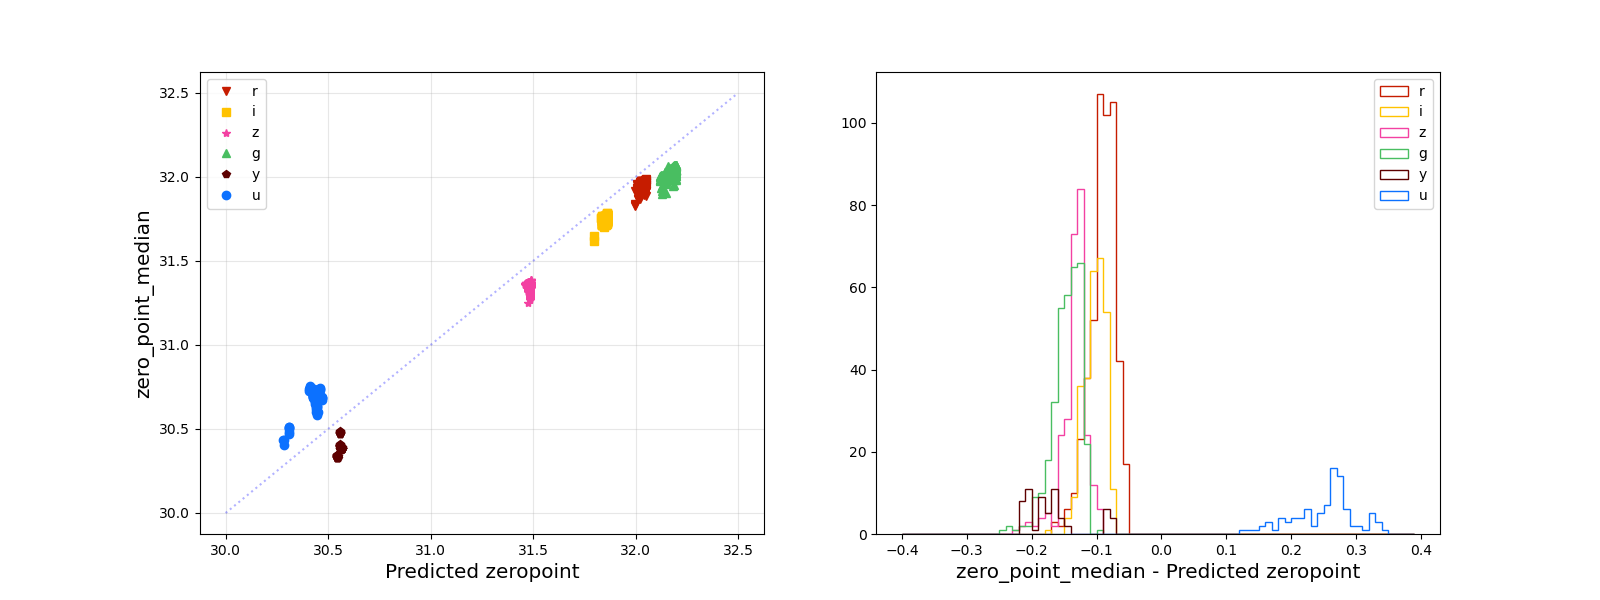
\includegraphics[width=0.8\textwidth]{sp/zeropoints.png}
    \caption{Predicted zeropoints from syseng\_throughputs (accounting for airmass) compared to measured zeropoints from `cdb\_lsst.comcam.visits1\_quicklook`.}
    \label{fig:zeropoints}
    \end{figure}
    
    
    
Likewise, the survey simulations use a skybackground model as part of the model to determine five sigma visit depths and to choose observation pointings. The outputs available in the ConsDb include a `sky\_bg\_median` value, which is in counts per pixel. Together with an estimate of the platescale (0.2"/pixel) and a zeropoint, we can convert this into magnitudes per square arcsecond, to compare to the predicted values from the rubin\_scheduler skybrightness model. The results are shown in Figure~\ref{fig:sky}.  The values are also remarkably consistent, with a scatter of less than 0.15 magnitudes in all bands, and offsets within 0.1 magnitude except in y band, where the measured sky is 0.5 magnitudes brighter than expected. This is  within our expected errors in the skybackground model, particularly in y band where the sky is quite variable and harder to model. 

\begin{figure}
    \centering
    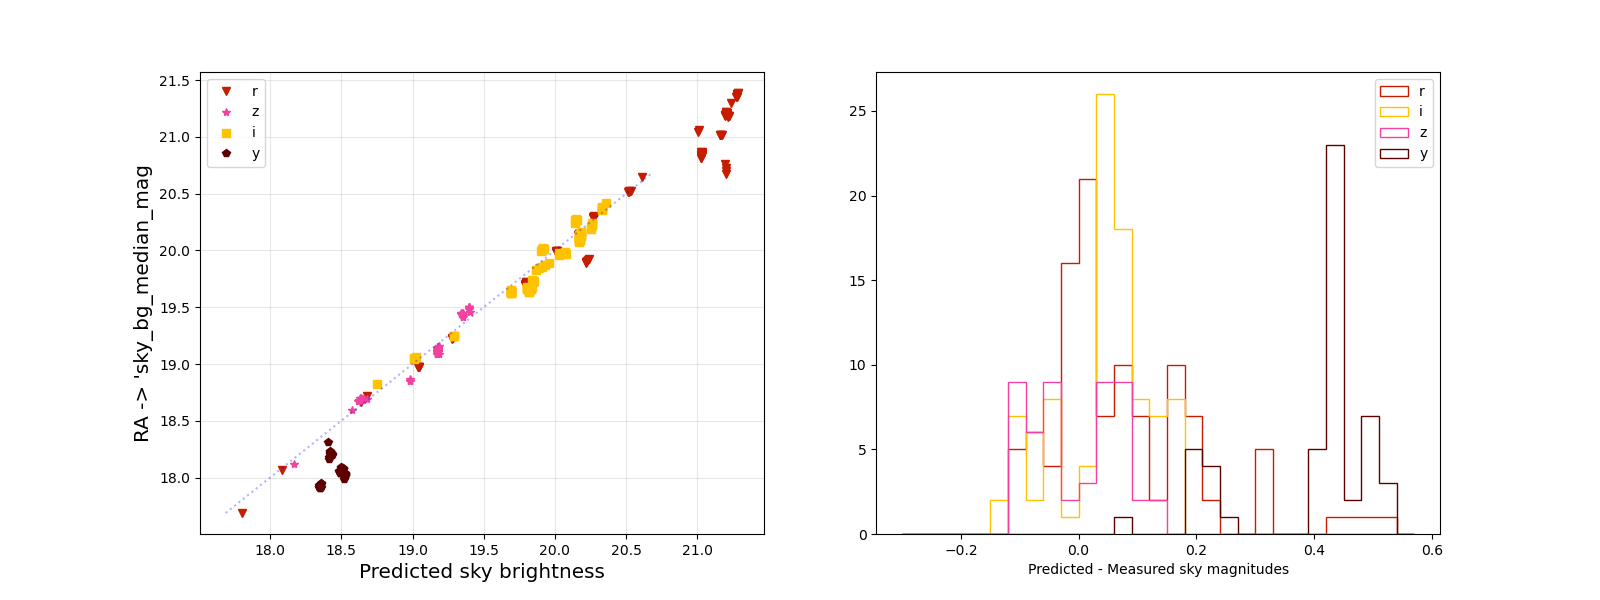
\includegraphics[width=0.8\textwidth]{sp/sky.png}
    \caption{Predicted skybrightness values from `rubin\_sim.skybrightness`  compared to `sky\_bg\_median` converted to mags per sq arcsecond  from  from `visits1\_quicklook`.}
    \label{fig:sky}
    \end{figure}
    
  
We look forward to comparing seeing performance to survey predictions. Initial estimates indicate that the mean seeing for these visits was around 1.12 arcseconds, which isn't out of line with longer term survey expectations, especially given that we remain in the early stages of commissioning. 

\begin{figure}
    \centering
    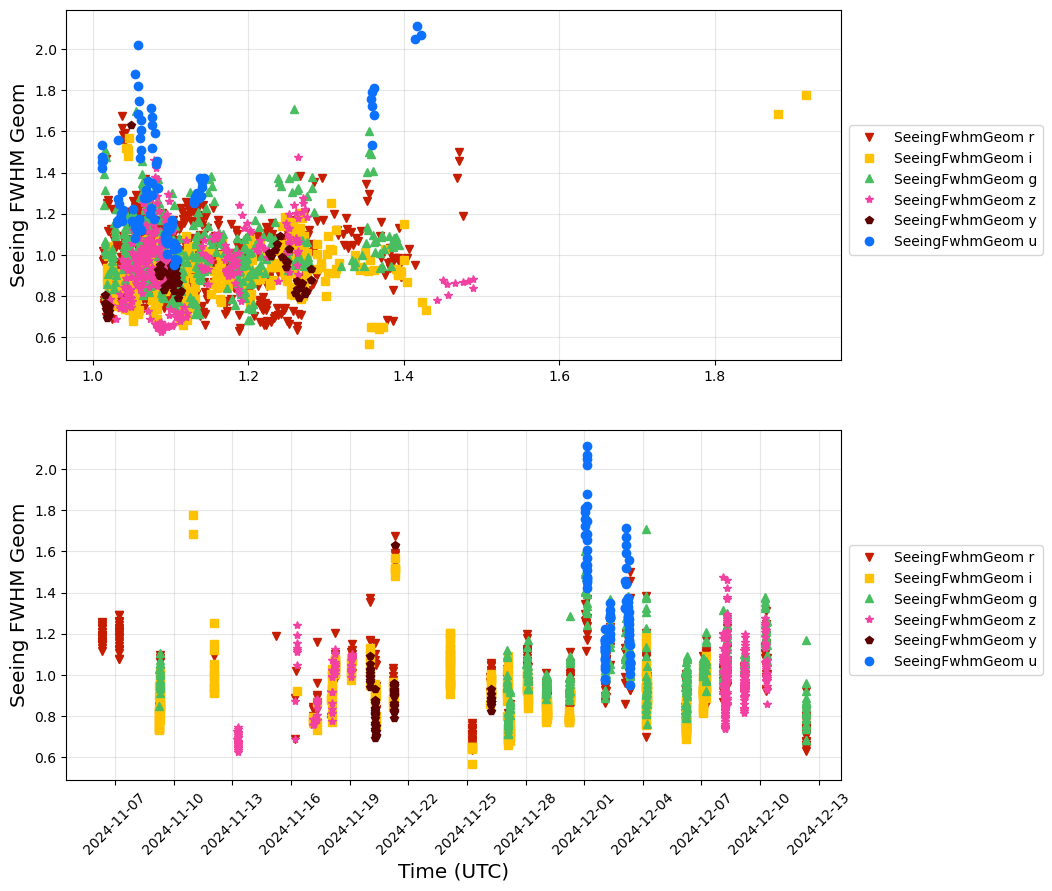
\includegraphics[width=0.8\textwidth]{sp/seeing.png}
    \caption{Converting `psf_sigma_median` into the single-gaussian effective seeing PSF values.}
    \label{fig:seeing}
    \end{figure}
    
   
Remaining questions include the efficiency of observations, and in particular the likelihood of whether a single snap will be sufficient. 